\documentclass[a4paper, 11pt]{article}

\usepackage{geometry}
\usepackage{setspace}
\usepackage{amsmath}
\usepackage{graphicx}
\usepackage{wrapfig}
\usepackage{caption}

\geometry{left=2.5cm, right=2.5cm, top=2.5cm, bottom=3cm}
\graphicspath{ {./images/} }
\newcommand{\ode}{{\fontfamily{pcr}\selectfont ode45()}}
\newcommand{\fft}{{\fontfamily{pcr}\selectfont fft()}}
\newcommand{\ifft}{{\fontfamily{pcr}\selectfont ifft()}}
\newcommand{\guessi}{{\fontfamily{pcr}\selectfont guess(i)}}
\newcommand{\guessii}{{\fontfamily{pcr}\selectfont guess(i + 1)}}
\newcommand{\guessiii}{{\fontfamily{pcr}\selectfont guess(i + 2)}}
\newcommand{\resi}{{\fontfamily{pcr}\selectfont result(i)}}
\newcommand{\resii}{{\fontfamily{pcr}\selectfont result(i + 1)}}
\newcommand{\dydt}{\frac{dy}{dt}}
\newcommand{\overm}[1]{\frac{#1}{m}}
\newcommand{\w}{$\omega$}
\newcommand{\m}{$\mu$ }
\newcommand{\shooting}{\textit{shooting} }
\newcommand{\Shooting}{\textit{Shooting} }
\newcommand{\arr}{\textit{array} }



\begin{document}
	
	\begin{figure}[t]
		
\includegraphics[scale=0.2]{Logo_UA}
	\end{figure}

	\title{Trabalho 2 - Oscilador não-linear \\ 
		{\Large Método de \Shooting e Transformadas de Fourier} \\
		{\large Física Computacional}}
	\author{João Inácio, 93039, PL7}
	\date{27/05/2020}
	\maketitle
	
	\section{Sumário}
	\paragraph{}
	O objetivo principal deste trabalho é estudar o movimento de um oscilador não-linear com recurso ao método da secante aplicado ao \shooting e a transformadas de Fourier (FT, do inglês \textit{Fourier Transform}). Na parte A do trabalho o objetivo é encontrar o parametro \m através do primeiro método e na parte B estudar a aceleração com recurso ao segundo método, FT. Usou-se o método \ode para fazer todas as integrações numéricas neste trabalho.
	No desenvolvimento do trabalho houve concordância entre os resultados esperados e os obtidos de cada um dos métodos, excepto no final do trabalho que as acelerações calculadas com recurso ao método \fft têm erros de aproximação.
	
	{\small Nota: Todos os gráficos e resultados foram obtidos através dos \textit{scripts} de MatLab presentes em anexo com este relatório. Alguma explicação dos códigos pode ser encontrada em comentário.}
	\section{Introdução}
	\paragraph{}
	A equação diferencial de movimento do oscilador não-linear é a seguinte
	\begin{equation}
		m\frac{d^2y}{dt^2}+K(y+\beta y^3)=\mu \left[1-\left( \dydt \right)^{2} \right]\dydt
	\end{equation}
	
	Para esta poder ser resolvida numéricamente pela rotina \ode do MatLab, é preciso dividi-la em duas equações diferenciais ordinárias (ODE, do inglês \textit{Ordinary Differential Equation}) de primeira orem. Assim se $\dydt=v$, temos as equações $(2)$ e $(3)$ 
	\begin{equation}
	\dydt = v 
	\end{equation}
	\begin{equation}
	\frac{dv}{dt} =  \overm{\mu} \left[1-\left(v\right)^{2} \right]v-\overm{K}(y+\beta y^3)
	\end{equation}
	que são duas ODE's de primeira ordem e podem ser usadas pela rotina \ode para a integração numérica.
	
	{\footnotesize Nota: Resposta à alínea a).}
	
	\subsection{Método de \Shooting}
	\paragraph{}
	O método de \shooting é um método numérico que resolve problemas de valor de fronteira através da redução do sistema a um problema de valores iniciais. Este método também é útil na eventualidade de ser necessário encontrar um parâmetro desconhecido, por exemplo um coeficiente da ODE, sabendo que um dos valores de fronteira tem de ser de tomar um certo valor.
	
	Para tal efeito, é preciso, em primeiro lugar, arbitrar duas estimativas, {\fontfamily{pcr}\selectfont guess(1)} e {\fontfamily{pcr}\selectfont guess(2)}, para o valor inicial ou o parâmetro que é pretendido encontrar. Estas duas primeiras suposições têm de ser próximas uma da outra no contexto do problema.
	
	Em segundo lugar é necessário assumir que o valor a ser encontrado toma a forma de \guessi, a primeira das estimativas, e integrar a expressão numéricamente, neste caso foi usado a rotina \ode.
	
	Por fim, na próxima iteração, é preciso verificar se o resultado proveniente da integração, \resi, ou seja, o valor de fronteira, satisfaz o valor pretendido e calcular uma nova estimativa, \guessii. Este calculo faz-se de acordo com o método da secante
	\begin{equation}
		m = \frac{\resi - result(i - 1)}{\guessi - guess(i - 1)}
	\end{equation}
	\begin{equation}
		b = \resi - m . \guessi
	\end{equation}
	
	De seguida podemos cacular a nova estimativa por
	\begin{equation}
		guess(i + 1) = guess(i) + \frac{B - result(i)}{m}
	\end{equation}
	onde $B$ é o valor de fronteira pretendido. Este processo de estimativas só para quando o valor absoluto da diferença de duas suposições seguidas for menor do que o erro especificado, {\fontfamily{pcr}\selectfont tol}.
	
	\subsection{Método da Secante}
	\paragraph{}
	Dadas duas estimativas, $x_{1}$ e $x_{2}$, para o zeros de uma função $f(x)$, o método da secante encontra $x_{0}$, tal que $f(x_{0})=0$. No caso a estudar, as duas estimativas são {\fontfamily{pcr}\selectfont guess(1)} e {\fontfamily{pcr}\selectfont guess(2)}, o valor que queremos encontrar, $x_{0}$, é o valor aproximado da condição inicial ou do parametro e a função $f$ é {\fontfamily{pcr}\selectfont result} em função de {\fontfamily{pcr}\selectfont guess}. Contudo, neste caso não se pretende encontrar $f(x)=0$, mas sim $f(x)=B$, ou seja, o valor de {\fontfamily{pcr}\selectfont guess} quando {\fontfamily{pcr}\selectfont result} é $B$. Para uma função $f(x)$ genérica a expressão de $x_{i+1}$ é
	\begin{equation}
		x_{i+1} = x_{i} + \frac{B-f(x_{i})}{m}
	\end{equation}
	onde $m$ é o declive da secante ao gráfico de $f$ e que passa em $x_{i+1}$ e $x_{i}$ e pode ser calculado por
	\begin{equation}
		tg(\alpha)=m=\frac{f(x_{i+1})-f(x_{i})}{x_{i+1}-x_{i}}
	\end{equation}
	As equações para o problema em questão são as equações $(4)$ e $(6)$.
	\newline
	{\footnotesize Nota: Parte da resposta à alínea d).}
	\newpage
	
	\section{Métodos e Resultados}
	\paragraph{}
	\subsection{Parte A - Método de \Shooting}
	\paragraph{}
	Para implementar o método de \shooting foram apresentadas duas estimativas para o valor de \m, {\fontfamily{pcr}\selectfont guess(1)}$= 1.4$ e {\fontfamily{pcr}\selectfont guess(2)}$= 1.6$ já que o valor real de \m é aproximadamente $1.5$. De seguida, fez-se um ciclo {\fontfamily{pcr}\selectfont for} para poder ser feito o \shooting {\fontfamily{pcr}\selectfont i} vezes até o parametro ter um erro menor que {\fontfamily{pcr}\selectfont tol}$=10^{-12}$. Foi integrada a ODE numéricamente com recurso à rotina \ode e encontrados os máximos de $y(t)$ para o dado parametro de \m.
	
	Para encontrar tais máximos usou-se a função {\fontfamily{pcr}\selectfont lagr.m}, que dado 3 pontos em que o ponto médio é o máximo numérico, encontra o ponto máximo da função contínua. Todos os pontos máximos da função foram colocados num \textit{array}, {\fontfamily{pcr}\selectfont A}, bem como os índices dos respetivos valores, num \textit{array} {\fontfamily{pcr}\selectfont idx}. Para obter uma melhor aproximação, foi calculada uma média aritmética de todos os máximos de $y(t)$ para ser comparado com o resultado esperado, $B=y_{max}=1.3$, ou seja, \resi=$\text{\textit{média}}(${\fontfamily{pcr}\selectfont A}$)$.
	
	Finalmente, é calculado o $m$ e \guessii, com recurso ao método da secante (secção 2.2), equações $(4)$ e $(6)$, respetivamente. Isto é feito até que, como já foi mencionado, o módulo da diferença entre duas estimativas seguidas, ou seja, $|$ \guessii$ - $\guessi $|$, tem de ser menor do que {\fontfamily{pcr}\selectfont tol}$=10^{-12}$.
	
	Para calcular o período de oscilação, o \textit{array} {\fontfamily{pcr}\selectfont idx} foi precorrido e com o uso da função {\fontfamily{pcr}\selectfont lagr.m} foi calculado o tempo de cada um dos máximos e foi armazenada num vetor {\fontfamily{pcr}\selectfont T} a diferença do tempo entre dois máximos consecutivos. Por fim, o período de oscilação é a média de todos os períodos.
	\newline
	{\footnotesize Nota: Estes parágrafos anteriores são a segunda parte da resposta para a alínea d).}
	\begin{wrapfigure}{r}{0.6\textwidth}
		\centering
		\captionsetup{labelformat=empty}
		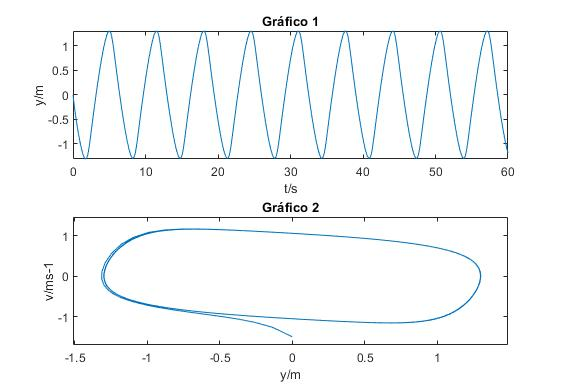
\includegraphics[scale=0.5]{parteA}
		\caption{\scriptsize Figura 1: gráfico 1 representa o movimento do oscilador em função do tempo, $y(t)$, o gráfico 2 representa o espaço de fases do oscilador.}
	\end{wrapfigure}
	\paragraph{}
	Deste modo, os valores de \m e do período, $T$, para uma amplitude positiva de $1.3$, são $\mu=1,88$ e $T=6,52s$. Também se pode ver nos gráficos 1 e 2, figura ao lado, o deslocamento em função do tempo e o espaço de fases para este oscilador não-linear.
	\paragraph{}
	Através de ambos os gráficos, verifica-se que o movimento do oscilador é periódico, com o período descrito a cima. Podemos ver também no gráfico 2 que ao longo do tempo, depois do movimento se estabilizar, o espaço de fases converge para um atrator de forma elíptica, figura 2, de centro $(0, 0)$, como é indicado pelo ponto azul.
	\paragraph{}
	\begin{wrapfigure}{l}{0.6\textwidth}
		\centering
		\captionsetup{labelformat=empty}
		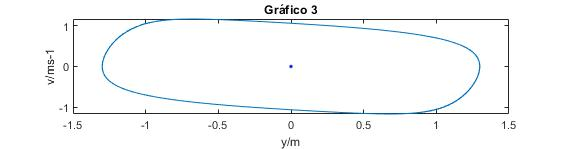
\includegraphics[scale=0.4]{atrator}
		\caption{\scriptsize Figura 2: gráfico 3 representa o atrator do espaço de fases do oscilador não-linear, o ponto azul representa o centro do atrator, $(0, 0)$.}
	\end{wrapfigure}
	Para fazer o gráfico 3, foram utilizados apenas os últimos 300 pontos de $y$ e $v$, uma vez que para pontos de t pequeno, o oscilador ainda estava a estabilizar o seu movimento harmónico.
	\newline
	\newline
	\paragraph{}
	Em relação à parte A do trabalho podemos concluir que para o parametro \m determinado, $\mu=1,88$, pelo método de \shooting temos um movimento periódico, com $T=6,52s$, que apesar de haver uma força dissipadora, coeficiente de $v$, há também uma força restauradora, $\beta y^3$, que faz com que não haja perdas de energia, tal como é mostrado no espaço de fases, ou seja, para $\mu=1,88$, há um equilíbrio nas forças, $F_{restauradora}=F_{dissipadora}$.
	\newline
	{\footnotesize Nota: Estes parágrafos a cima respondem às questões b) e c).}
	
	\subsection{Parte B - Transformadas de Fourier}
	\paragraph{}
	Para estudar o movimento do oscilador com o uso de transformadas de Fourier, é usado o método \fft, uma função do MatLab que usa o algoritmo \textit{fast fourier transform}. Este método não calcula FT, $F(\omega)$, por si, calcula sim a transformada discreta de Fourier (DFT, do inglês \textit{Discrete Fourier Transform}), $F(k)$, e a inversa usando \ifft. FT e DFT estão relacionadas da seguinte forma
	\begin{equation}
		F(\omega)=\Delta t F(k)
	\end{equation}
	A densidade espectral pode ser calculada da seguinte forma
	\begin{equation}
		Densidade\ Espectral = \left| F(\omega) \right|^{2}
	\end{equation}
	No caso da derivação da função TF, a relação é a seguinte equação
	\begin{equation}
		\frac{d^{n}f(t)}{dt^{n}}=(i\omega)^{n}F(\omega)
	\end{equation}
	A transformada de Fourier passa uma função de domínio $t$ para uma função de domínio $\omega$. O algoritmo \fft calcula $F(k)$, de uma maneira eficiente e rápida, dado o nome, visto que tem uma complexidade computacional de $\mathcal{O}(N\log{N})$, $N$ é o número de elementos do \arr de posições.
	\paragraph{}
	Para implementar o código desta questão, em primeiro lugar, usando um vetor de tempo com comprimento igual a 1024, $N$, e com um passo $dt=0.1$, foi criado um vetor de frequências angulares $\omega$ para o domínio de TF. As fórmulas para calcular os extremos e passo desse vetor são
	\begin{equation}
		d\omega=\frac{2\pi}{Ndt}
	\end{equation}
	\begin{equation}
		\omega_{max} = \left(\frac{N}{2} - 1\right)d\omega
	\end{equation}
	\begin{equation}
		\omega_{min} = -\frac{N}{2}d\omega
	\end{equation}
	Com as últimas três equações, criou-se o vetor de frequências. De seguida, foram resolvidas numéricamente as equações (2) e (3), pela rotina \ode.
	\newline
	\paragraph{}
	Seguidamente, foi usado a função \fft para determinar a DFT, {\fontfamily{pcr}\selectfont fftshit()} para centrar os valores da DFT e, por fim, isto foi multiplicado por $dt$ para obter $F(\omega)$, como dita a relação (9). Foi calcula da densidade espectral de acordo com a equação (10) e daí resultou a seguinte figura, 
	\newline
	{\footnotesize Nota: Estes parágrafos a cima correspondem a metade da resposta à questão g).}
	\begin{figure}[h]
		\centering
		\captionsetup{labelformat=empty}
		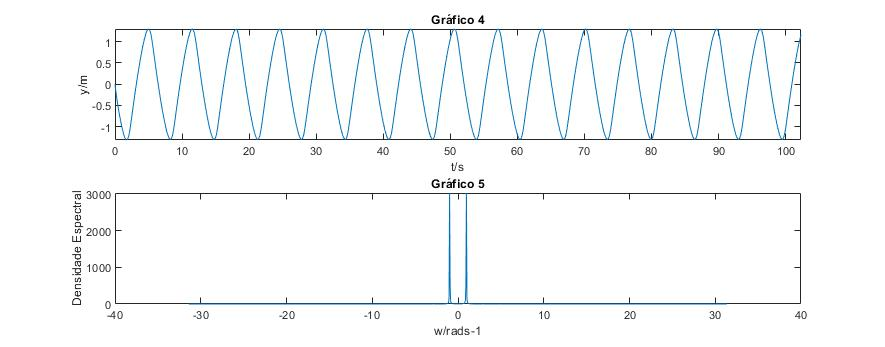
\includegraphics[scale=0.4]{parteB_1}
		\caption{\scriptsize Figura 3: gráfico 4 representa o deslocamento, $y$, do oscilador em função do tempo, o gráfico 5 representa a densidade espectral em função do domínio das frequências.}
	\end{figure}
	\paragraph{}
	Pela observação do gráfico 5, podemos concluir, mais uma vez, que o movimento do oscilador é de facto periódico, já que no domínio de frequências, a função apresenta um pico à volta de $\omega=1$, e o seu simétrico em $\omega=-1$. Ou seja, o sistema oscila apenas com uma e uma só frequência. O calculo do período associado a esta frequência vai ser calculado mais a baixo para comparar com o valor encontrado na secção 3.1.
	\newline
	{\footnotesize Nota: Este parágrafo a cima corresponde à resposta da alínea e).}
	\paragraph{}
	Para poder ser mais fácil a comparação da frequência máxima, temos de ampliar o gráfico, ou seja, diminuir $d\omega$ por um fator de 4. Para tal, multiplicou-se o valor de $dt$ por 4, já que segundo a fórmula (12) $d\omega$ é proporcional a $\frac{1}{dt}$. Com esta alteração foi calculado outra vez um vetor de frequências e feito e a densidade espectral da mesma forma descrita a cima.
	\paragraph{}
	Como os pontos máximos da densidade espectral estão próximos de 3000, é pedido para considerar pontos cuja densidade espectral é menor do que 10. Assim, foi usado uma sintaxe do MatLab que permite escolher os índices dos pontos de um \arr que têm um determinado valor com o intuito de ir buscar os valores associados a esses índices noutro \arr. Exemplo:
	\paragraph{}
	Supor que se tem os seguintes vetores {\fontfamily{pcr}\selectfont a = [1, 2, 4, 8]}, {\fontfamily{pcr}\selectfont b = [4, 8, 10, 11]} e  {\fontfamily{pcr}\selectfont c}, definido por {\fontfamily{pcr}\selectfont c = a(b < 9)}. A operação {\fontfamily{pcr}\selectfont (b < 9)} vai buscar os índices dos valores de {\fontfamily{pcr}\selectfont b} que são maiores do que 9, logo {\fontfamily{pcr}\selectfont (b < 9) = [3, 4]}. Desde modo, {\fontfamily{pcr}\selectfont c} são os valores de {\fontfamily{pcr}\selectfont a(3)} e {\fontfamily{pcr}\selectfont a(4)}, {\fontfamily{pcr}\selectfont c = [4, 8]}.
	\paragraph{}
	Este método foi usado para encontrar as frequências cuja densidade espectral associada é menor do que 10. Foi feito um {\fontfamily{pcr}\selectfont plot()} destas frequências e densidades espectrais, assim temos a figura 4. 
	\newline
	{\footnotesize Nota: Estes parágrafos correspondem ao resto da questão g).}
	\begin{figure}[h]
		\centering
		\captionsetup{labelformat=empty}
		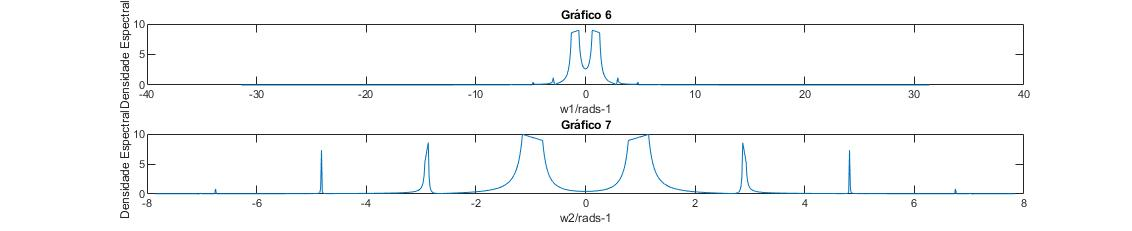
\includegraphics[scale=0.4]{parteB_2}
		\caption{\scriptsize Figura 4: gráficos 6 e 7 correspondem às densidades espectrais menores que 10 em função das frequências. O gráfico 7 tem uma resolução 4 vezes maior.}
	\end{figure}
	\paragraph{}
	Analisando ambos os gráficos verificar-se que já não há só uma frequência que sobressalta, em vez disso temos 4. Isto pode ser devido a erros de arredondamento no método \fft, já que estas frequências estão numa densidade espectral de 10, enquanto as outras numa ordem de 3000. Se for calculado o período ($T=\frac{2\pi}{\omega}$) associado ao primeiro e segundo pico no gráfico ($\omega=0.7823$ e $\omega=1.15$), obtemos um intervalo $[5.46, 8.03]$ em que o período determinado em 3.1 ($T=6.52$) pertence. Ou seja, o movimento é sim periódico, os gráficos apenas têm erros de arredondamento devido algoritmo \fft. 
	\newline
	{\footnotesize Nota: Este parágrafo corresponde à resposta à questão f).}
	\paragraph{}
	Por fim, foi calculada a velocidade através da TF usando a relação das derivadas, equação (11) e usando {\fontfamily{pcr}\selectfont y} e {\fontfamily{pcr}\selectfont v} determinados pela \ode, que foi calculado através da equação (1), já que $a=\frac{d^2y}{dt^2}$. Resultou a figura 5.
	\begin{figure}[h]
		\centering
		\captionsetup{labelformat=empty}
		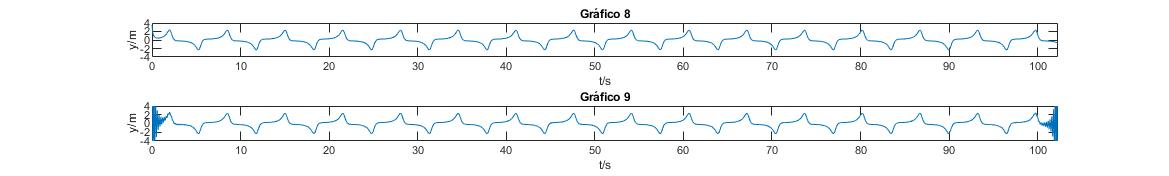
\includegraphics[scale=0.4]{parteB_3}
		\caption{\scriptsize Figura 5: gráficos 8 e 9 representam a aceleração em função do tempo. O gráfico 8 foi feito através dos cálculos da \ode e o 9 através da derivada de FT.}
	\end{figure}
	\paragraph{}
	Ambos os gráficos estão muito parecidos o que indica que quer pela \ode que por FT se pode calcular a aceleração de uma forma correta, contudo para os extremos de tempos, o gráfico 9 tem ruído, o que indica que há pequenos erros de arredondamentos e aproximações no que toca a fazer a transformada de Fourier inversa. 
	\newline
	{\footnotesize Nota: Estes dois parágrafos correspondem à resposta à questão h).}
	\section{Discussão e Conclusão}
	\paragraph{}
	A maioria dos resultados foram precisos, com excepção dos dois últimos gráficos da parte B. Esses erros podem estar associados e erros de truncatura e arredondamento dentro do algoritmo \textit{fast fourier transform} que o MatLab usa.
	\paragraph{}
	Em suma, foi estudado o movimento do oscilador não-linear com recurso ao método de \shooting e \fft, foi determinado o valor de \m quando a amplitude máxima positiva é 1.3, o valor do período e a aceleração de duas formas, chegando à conclusão que se trata de um oscilador periódico para $\mu=1.88$.
	
	
	
	
	
	
	
	
\end{document}